\chapter*{Otras funciones elementales}
\setcounter{chapter}{1}
\setcounter{section}{0}

\section{Funciones homográficas}
Las funciones homográficas son \emph{funciones racionales} de la forma
$$f : A \subseteq \R \rightarrow B \subseteq \R / f(x) = \frac{p(x)}{q(x)}$$
donde $p$ y $q$ son polinomios

\blueBox{Definición - Función homográfica}{
    Se llama función homográfica a las funciones de la forma: 
    $$f(x) = \frac{ax + b}{cx + d} \text{ donde } c \neq 0 \text{ y } ad-bc \neq 0$$
}
El caso más elemental es cuando $a = d = 0$ y $b = c = 1$ y se llama \emph{función identidad}.
$$f(x) = \frac{1}{x}$$
Como el denominador no puede ser igual a 0, el dominio es:
$$Dom(f) = \R - {0}$$
\begin{center}
    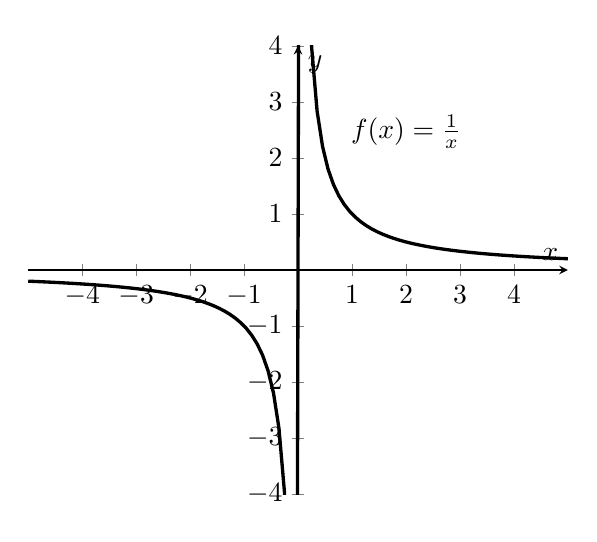
\begin{tikzpicture}
        \begin{axis}[
            xmin=-5, xmax=5,
            ymin=-4, ymax=4,
            axis lines=middle,
            xtick={ -4, -3, -2, -1, 0, 1, 2, 3, 4},
            ytick={ -4, -3, -2, -1, 0, 1, 2, 3, 4},
            xlabel=$x$,
            ylabel=$y$,
            legend pos=north west,
            legend cell align=left,
            ]
            \addplot[domain=-5:5, samples=100, color=black, very thick] {1/x};
            % nodes for the functions
            \node[above] at (axis cs:2, 2) {$f(x) = \frac{1}{x}$};
        \end{axis}
    \end{tikzpicture}
\end{center}
La gráfica se conoce como \emph{hipérbola} y tiene las siguientes características.
\begin{enumerate}
    \item {A medida que se acerca al 0, y es cada vez más grande\\
        Decimos que la función \emph{tiende a más infinito} cuando $x$ tiene a 0 desde la derecha:
        $$f(x) \rightarrow +\infty \text{ cuando } x \rightarrow 0^+$$
        Decimos que la función \emph{tiende a menos infinito} cuando $x$ tiene a 0 desde la izquierda:
        $$f(x) \rightarrow -\infty \text{ cuando } x \rightarrow 0^-$$
        La función tiene \emph{asíntota vertical} en $x = 0$.
    }
    \item {Por otro lado, cuando x es cada vez más grande, y es cada vez más pequeño\\
        Decimos que la función \emph{tiende a 0} cuando $x$ tiene a $\pm \infty$:
        $$f(x) \rightarrow 0 \text{ cuando } x \rightarrow \pm \infty$$
        La función tiene \emph{asíntota horizontal} en $y = 0$.

    }
\end{enumerate}
Todas las funciones homográficas tienen las mismas características.
\begin{enumerate}
    \item Sus gráficas son hipérbolas
    \item Tienen asíntota vertical
    \item Tienen asíntota horizontal
\end{enumerate}
Si la función es:
$$f(x) = \frac{ax + b}{cx + d}$$
La asíntota horizontal es:
$$y = \frac{a}{c}$$
y la vertical es:
$$x = -\frac{d}{c}$$

\section{Función módulo: $f(x) = |x|$}
Desde el punto de vista funcional, podemos pensar en una función que a los números negativos se les asigna como imagen el valor absoluto de ese número, y a los positivos se les asigna el mismo número.
$$f : \R \rightarrow \R / f(x) = |x| = 
\begin{cases}
    x & \text{si } x \geq 0 \\
    -x & \text{si } x < 0
\end{cases}
$$
% \begin{center}
%     \begin{tikzpicture}
%         \begin{axis}[
%             xmin=-5, xmax=5,
%             ymin=-1, ymax=4,
%             axis lines=middle,
%             xtick={ -2, -1, 0, 1, 2},
%             ytick={ 1, 2},
%             xlabel=$x$,
%             ylabel=$y$,
%             legend pos=north west,
%             legend cell align=left,
%             ]
%             \addplot[domain=-5:5, samples=100, color=blue, very thick] {abs(x)};
%             \node[above] at (axis cs:2, 2) {$f(x) = |x|$};
%         \end{axis}
%     \end{tikzpicture}
% \end{center}
Se puede desplazar la gráfica si se cambian los argumentos: 
$$f(x) = |x - a| - b$$
$a$ es la cantidad que cambia en el eje X y $b$ es la cantidad que cambia en el eje Y.

\section{Función raíz cuadrada: $f(x) = \sqrt{x}$}
Vimos que $x^2$ no tiene inversa, ya que no es biyectiva.\\
Para hacer la función inversa, hay que cambiar el dominio. En vez de considerar todos los números reales, vamos a considerar los números positivos.
$$f: \R_0^+ \rightarrow \R_0^+ / f(x) = x^2 $$
$$ f^{-1} : \R_0^+ \rightarrow \R_0^+ / f^{-1}(x) = \sqrt{x}$$

Características:
\begin{enumerate}
    \item Solo aplica a \textbf{números positivos} (su dominio es $\R_0^+$)
    \item Sus imágenes son positivas
    \item La gráfica se obtiene haciendo una simetría respecto al eje $y = x$ de la función $x^2$
    \item Es estrictamente creciente en el intervalo $[0; +\infty)$
\end{enumerate}

\begin{center}
    \includegraphics[width=0.7\linewidth]{img/sqrt(x).jpg}
\end{center}
